\providecommand{\topdir}{..}
\documentclass[../main.tex]{subfiles}

%External sources
\graphicspath{{\topdir/img/02/}}

\begin{document}
\label{chap:soa}

\section{Historical evolution of vision mixers}
The first vision mixers were introduced into the market as soon as the first commercial \gls{tv} broadcasters began operations in the mid 1930s. At that time, vision mixers operated in a mechanical manner, this is, they merely consisted of switch matrices used to route the input signals to the main output. As no signal processing was performed, all inputs needed to be \textit{genlocked}; In other words, their horizontal sync pulses needed to happen at the same time\cite{becg2020}.\newline

As time passed, these commutation matrices evolved into complex analog mixers, which allowed to perform several effects using analog electronics, although they still needed \textit{genlocked} sources. For instance, these mixers were able to fade or wipe between sources, or compose using \textit{luma key}s\cite{WardPeter2001Saob}. This same time, the standard program-preset operation model was introduced, as opposed to the older A-B model. The mixer displayed in the figure \ref{fig:02:piher} features both an A-B and a program-preview bank.\newline

\begin{figure}[htbp]
    \centering
    \subfigure{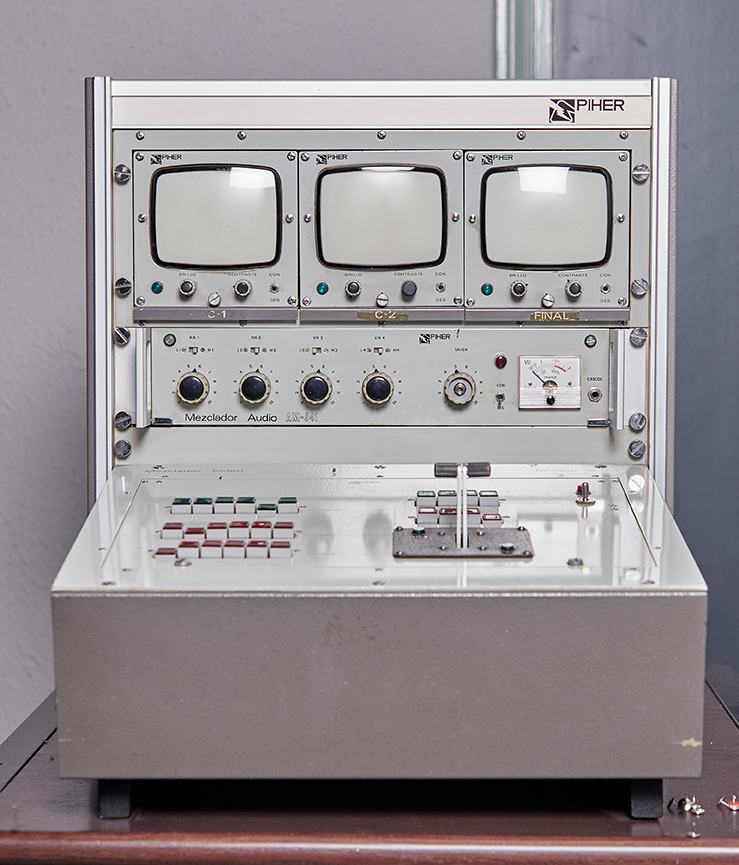
\includegraphics[height=6.5cm]{piher1}}
    \subfigure{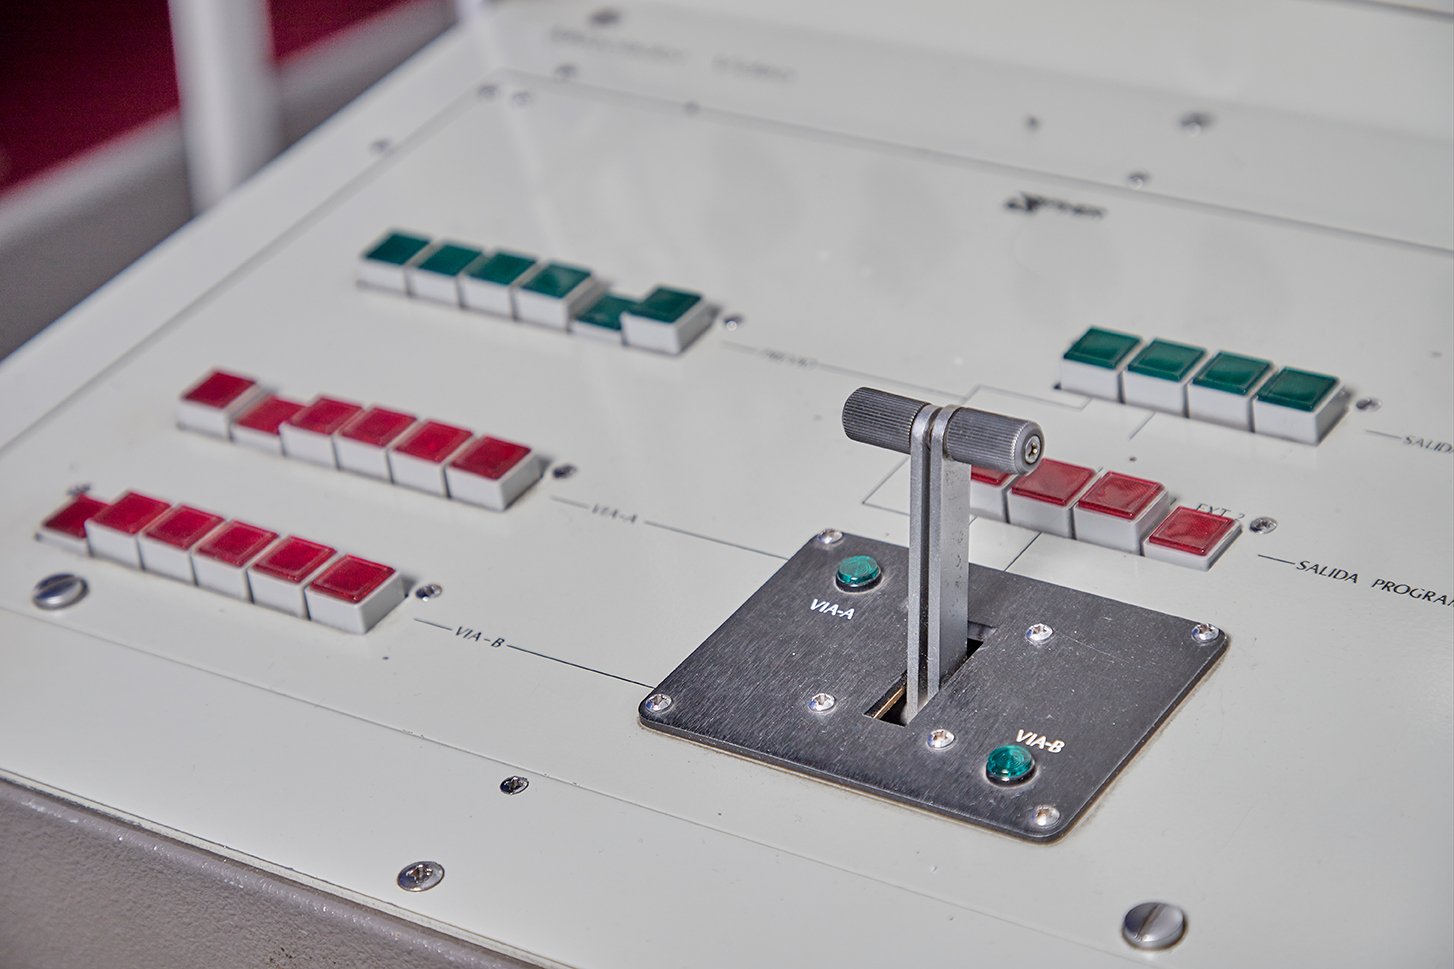
\includegraphics[height=6.5cm]{piher2}}
    
    \footnotesize{Photos by Facultad de Ciencias de la Información, Universidad Complutense de Madrid}
    \caption{Piher vision mixer, circa 1960}
    \label{fig:02:piher}
\end{figure}

Shortly after, in the late 1960s, some \gls{tv} stations began broadcasting colour signals. This implies that vision mixer technology needed to evolve to handle these new signals. The presence of colour was useful to introduce a powerful technique that is still used: \textit{chroma keying}\cite{jpeters}\cite{tmMixerHistory}. This gives the ability to delete parts of a frame based on its colour. It is typically used in weather forecasts; where the presenter sits in front of a green screen which gets replaced with a weather map by the vision mixer.\newline

Several years later, advancements in digital \gls{ic} manufacturing made possible to manipulate video digitally\cite{kitplus2015}. This introduced discrete digital effect processors, known as \glspl{dve}. These allowed spatial transformations of video frames, which were impractical with analog electronics, as high bandwidth signal delays would be needed. Shortly after, these discrete effect processors were integrated into the mixers. Nowadays, although the whole pipeline of the mixers is digital, the \gls{dve} term is still used to refer to those effects which involve spatial transformations of a frame\cite{OwensJim2020Tp}\cite{UtterbackAndrew2015STPa}.\newline

There was a short period in the late 1980s where all video processing was performed with digital electronics but the video \gls{io} was performed using analog signals by the means of \glspl{adc} and \glspl{dac}. This suddenly changed with the introduction of the \gls{sdi} communications protocol, which allows transmitting video alongside ancillary data over a $75 \si{\ohm}$ coaxial cable\cite{OrtizRodriguez2018}. This protocol is still used on its latest revision, which specifies a stream of $12 \si{\giga b \per\second}$. Moreover, it has been adapted to support other transmission mediums such as optical fiber.\newline

The latest advancements came in the late 2000s with the introduction of the first software-based mixers by NewTek. At this same time, the first \gls{ip} based production protocols were also introduced. In short terms, \gls{ip} based production replaces the dedicated coaxial cables with the more versatile Ethernet cables. These in turn can be twisted-pair shielded cables or optical fiber. \Gls{ip} based production and software-based mixers work well together, as they facilitate live video production with no dedicated broadcasting equipment.\newline


\section{Common vision mixer features}
Modern vision mixers usually integrate many simpler mixers, known as \gls{me} banks\cite{}. Each of these units is a full-fledged mixer, which will be responsible of generating a single composition. However, they might generate more than one distinct output signal for reasons that will be explained later. In rough terms, the category of a vision mixer can be measured by its amount of \gls{me} units, although this is quite simplistic, as the feature set of each one of these banks may be more important, but more often than not, there is a certain amount of linearity among these two specifications. Most mixers in the market have 1 to 4 \gls{me} units, topping out at 8.\newline

Each \gls{me} has a signal matrix known as the \textit{crosspoint}. It serves as a router for input signals, which are represented as columns. Meanwhile, each of the feeds required by the \gls{me} will be represented as a row, which can only be fed by one or zero input signals.\newline

\Glspl{me} are based on the program/preview operation model. This operation model consists in configuring the next composition in advance at the preview bus. Meanwhile, the program bus is permanently on air. When the time is right, the contents of the preview bus are swapped with the contents of the program bus, either by an instantaneous cut or a transition. Therefore, each \gls{me} generates two video signals: program and preview. This gives the operator the ability to double check for errors in the composition before it is broadcasted. However, manual changes in the program bus can be performed, although it is not a good operation practice, as any composition errors will be instantaneously transmitted.\newline

Each of these composition buses are founded on the background layer. This layer is always visible -although it may be black or transparent- and encompasses the whole screen. As suggested by its name, its only ability is to display a video signal in the background. If no compositing is required, it is used to display the main video feed.\newline

Several layers called \textit{keyers} may be hierarchically added on top of this background. Low-indexed \textit{keyers} can be occluded by higher indexed ones. Moreover, they can be classified as \glspl{usk} and \glspl{dsk}. The difference between these two is that \glspl{usk} are added before the transition generator, whilst \glspl{dsk} are added to the signal that has the transition already on it. If the transition is inactive, it can be considered that \glspl{dsk} have a higher priority, so they will occlude \glspl{usk}. Usually the \glspl{usk} are used to perform compositions that are background dependant. Meanwhile, the \glspl{dsk} are used to add more stationary contents, such as banners and \gls{tv} station watermarks. Therefore, most vision mixers offer more \glspl{usk} compared to the number of \glspl{dsk}. A possible case of each one of them is shown in the figure \ref{fig:02:usk_dsk_example}.

\begin{figure}[htbp]
    \centering
    
\includegraphics[width=.8\textwidth]{usk_dsk}

    Note: Both \glspl{usk} are \glspl{dve}. The \gls{dsk} is a linear keyer.
    \caption{Possible use case of USKs and DSKs}
    \label{fig:02:usk_dsk_example}
\end{figure}

A general view of the signal path of a hypothetical 8-input \gls{me} unit can be seen in the figure \ref{fig:02:me_signal_path}.\newline

\begin{landscape}
\begin{figure}[htbp]
    \centering
    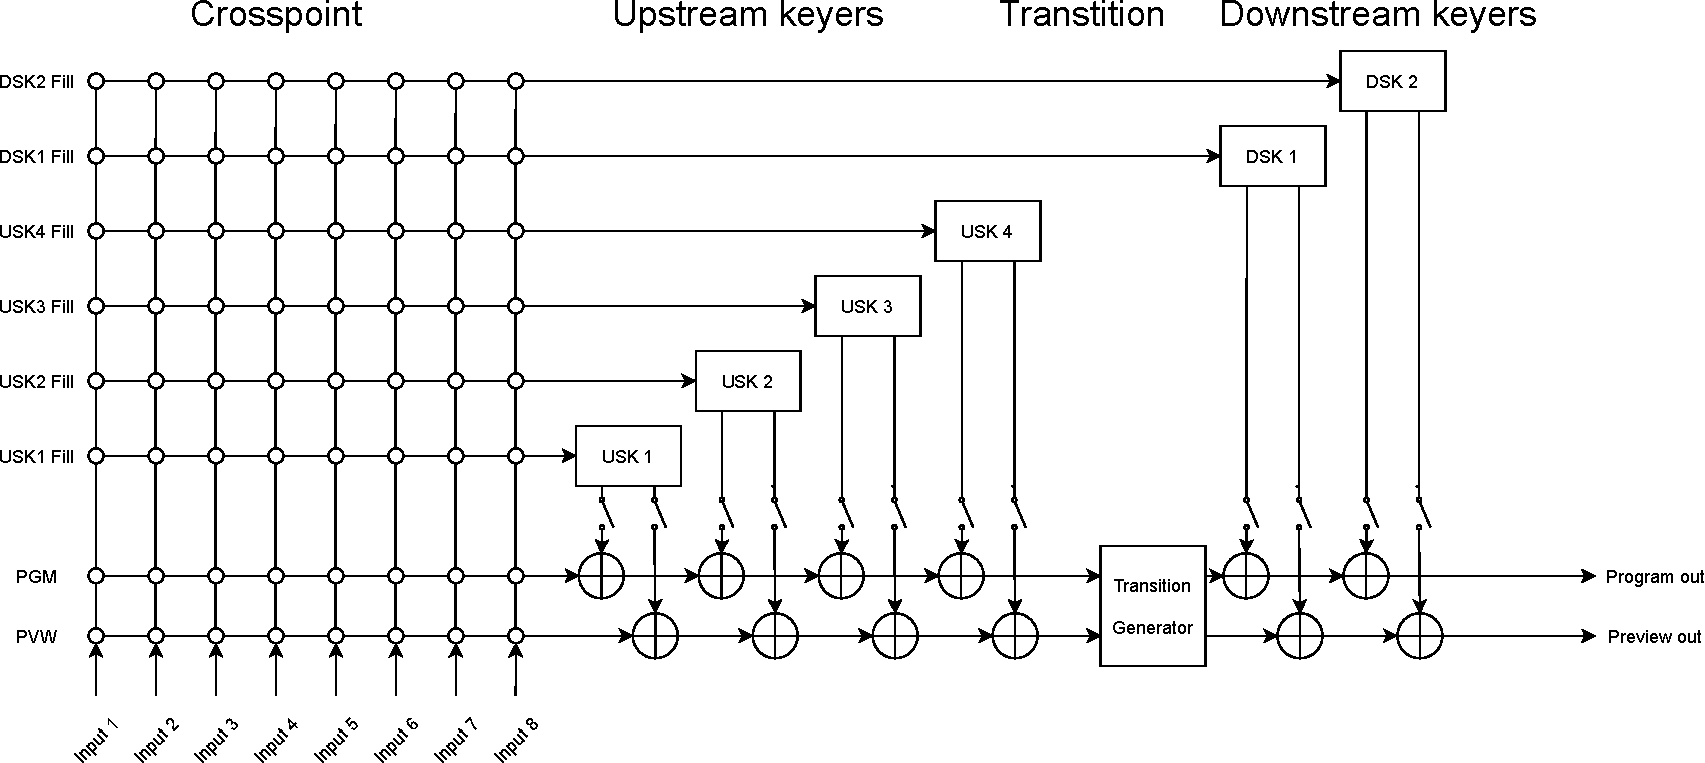
\includegraphics[width=\linewidth]{ME Block Diagram}

    \caption{Signal path of a hypothetical ME with 8 inputs, 4 USKs and 2 DSKs}
    \label{fig:02:me_signal_path}
\end{figure}
\end{landscape}

\subsection{Mixing equation}
Most of the effects performed by a vision mixer can be modelled using the equation \eqref{eq:mixing}, where $a$ is the background image and $b$ is the foreground image. These two images get weight-averaged using the control signal $c$ and its complementary. This control signal is also an image. Therefore, places where $c$ is high, the foreground image will predominate. The reverse is also true, if $c$ is low, the background image will predominate. In the context of digital image processing, this is a linear point operation.

\begin{equation} \label{eq:mixing}
    r(x, y) = (1 - c(x, y))  \cdot a(x, y) + c(x, y) \cdot b(x, y) \qquad c(x, y) \in [0, 1]
\end{equation}

To obtain colorimetrically correct results, $a$ and $b$ must be linear, this is, they must not contain a gamma correction. The most basic form of gamma correction is shown in the equation \eqref{eq:gamma} where $x'$ denotes the gamma corrected value and $x$ is the linear value. Typically, $\gamma$ equals $2.2$. Similarly, ITU-R described in the BT.1886 standard\cite{bt1886} the gamma transfer function that is shown in the equation \eqref{eq:bt1866}. These are not the only gamma corrections used in the industry, but they are the most important ones.\newline

\begin{equation} \label{eq:gamma}
    x = x'^{\gamma} \Longleftrightarrow x' = x^{\frac{1}{\gamma}} \qquad x, x' \in [0, 1]
\end{equation}

\begin{equation} \label{eq:bt1866}
    x =
    \begin{cases}
        \frac{x'}{4.5} &\text{if} \quad x' \le 0.081 \\
        (\frac{x' + 0.099}{1.099})^{\frac{1}{0.45}} &\text{otherwise}
    \end{cases}
    \Longleftrightarrow
    x' =
    \begin{cases}
        4.5x &\text{if}\quad x \le 0.018 \\
        1.099x^{0.45} - 0.099 &\text{otherwise}
    \end{cases}
\end{equation}

\subsection{Keying}
As mentioned earlier, keyers are used to overlay an image on top of the background. However, to be able to see that background, parts of the foregound image need to be conditionally transparent. The process of discriminating parts of the overlay is known as keying. Several techniques have been developed to achieve such a task, the most common of which will be explained hereunder.\newline

\subsubsection{Linear keying}
This is one of the oldest keying techniques. It consists in using a matte signal which represents the transparency of the filling signal. Considering the mixing equation \eqref{eq:mixing}, the background and fill images would be $a$ and $b$ respectively. Meanwhile, the matte signal would be equivalent to the control signal.\newline

If a signal carries its own matte information, it is said that it has an alpha channel. The most common usage of the linear key is to overlay \glspl{cg} or other types of computer generated graphics. For instance, the \gls{dsk} shown in the figure \ref{fig:02:usk_dsk_example} could be using this technique. Unlike other types of keying, it requires two video sources -apart from the background signal- as seen in the figure \ref{fig:02:linear_key_example}. Even though this example uses a binary matte signal -black or white-, it is worth noting that it supports gray-scale matte images which smoothly blend from the background image to the keyed image.\newline

\begin{figure}[htbp]
    \centering
    \subfigure[Fill image]{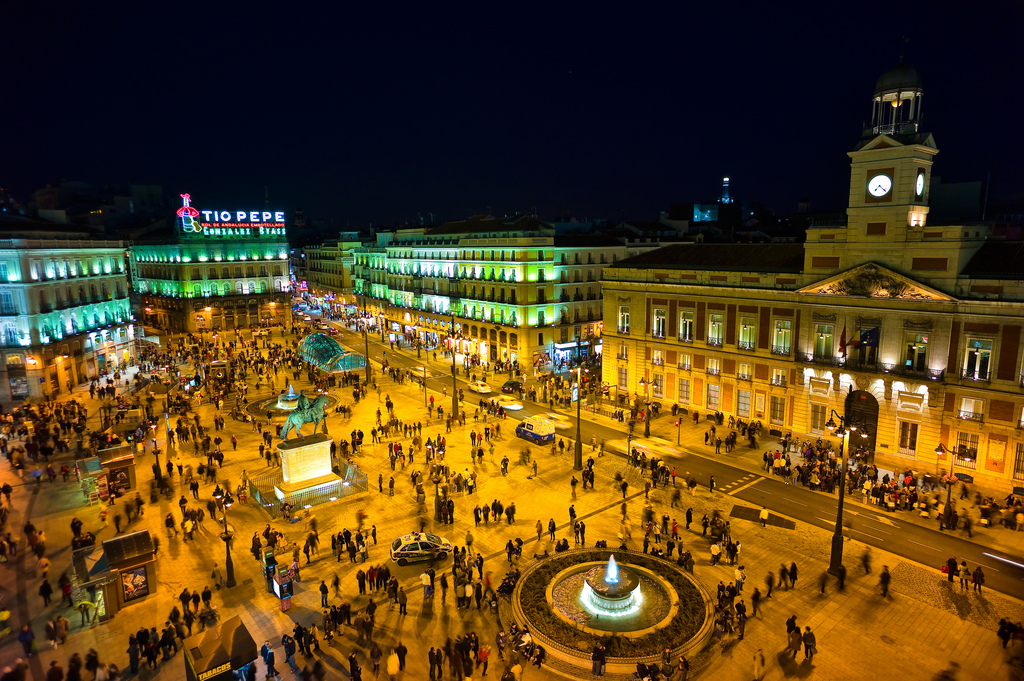
\includegraphics[height=3cm]{linear_fill}}
    \subfigure[Matte image]{
\includegraphics[height=3cm]{linear_key}}
    \subfigure[Linear keyed image]{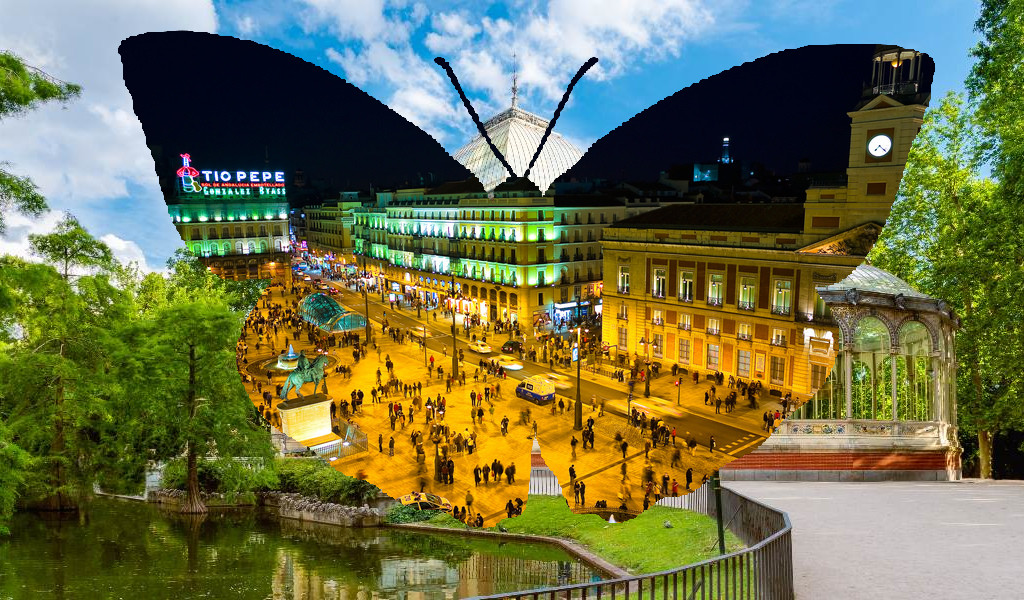
\includegraphics[height=3cm]{linear_comp}}

    \caption{Linear key example}
    \label{fig:02:linear_key_example}
\end{figure}

\subsubsection{Pattern keying}
This is similar to the previous type of keying. However, the matte signal is a internally generated preset. In the figure \ref{fig:02:patterns} a list of patterns offered by a commercial mixer can be observed.\newline

\begin{figure}[htbp]
    \centering
    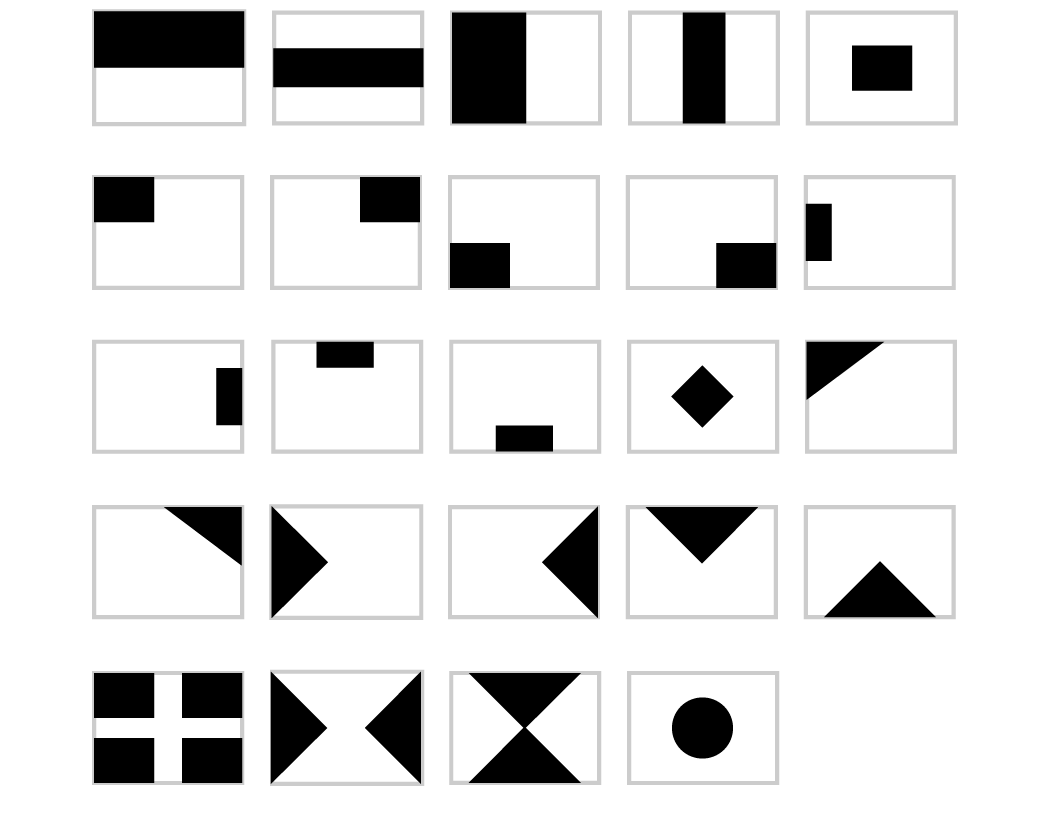
\includegraphics[width=.6\textwidth]{patterns}
    \caption{Patterns offered by Ross vision mixers}
    \label{fig:02:patterns}
\end{figure}

\subsubsection{Luma keying}
This type of keying is very similar to the linear key. However, instead of using a dedicated signal for transparency information, it uses the filling signal's own luminosity. Similarly to linear keying, $a$ and $b$ terms of the mixing equation \eqref{eq:mixing} would be the background and fill images, but the control signal would be a function of the filling singnal's luminance channel: $c(x, y) = f(Y(x, y))$, hence its name.\newline

This is only useful if the transparent parts are very black and opaque parts are very white or vice versa. Since the luminosity information can not be controlled separately, these keyers usually have more advanced settings that model the behaviour of the function that relates the luminance to the control image. Possible settings for this transfer function could be a lower and upper threshold, a toggle for inverting the result, etc\dots An example of this type of keying is displayed in the figure \ref{fig:02:luma_key_example}.

\begin{figure}[htbp]
    \centering
    \subfigure[Background image]{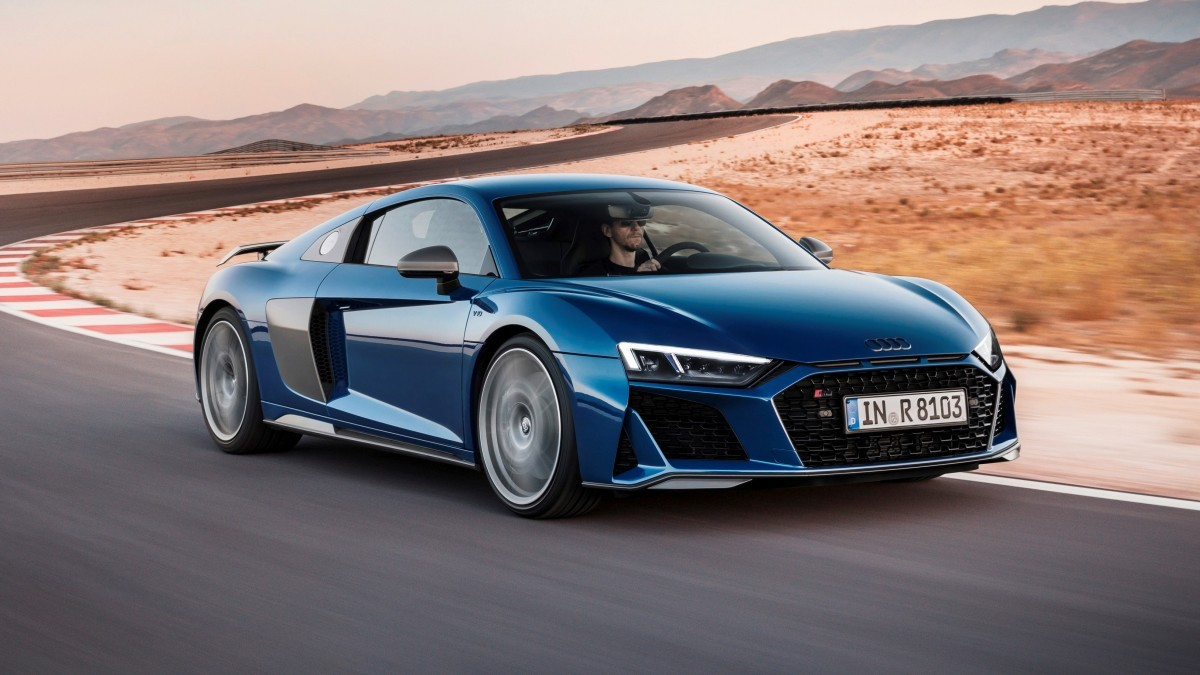
\includegraphics[height=2.8cm]{luma_bkgd}}
    \subfigure[Key source]{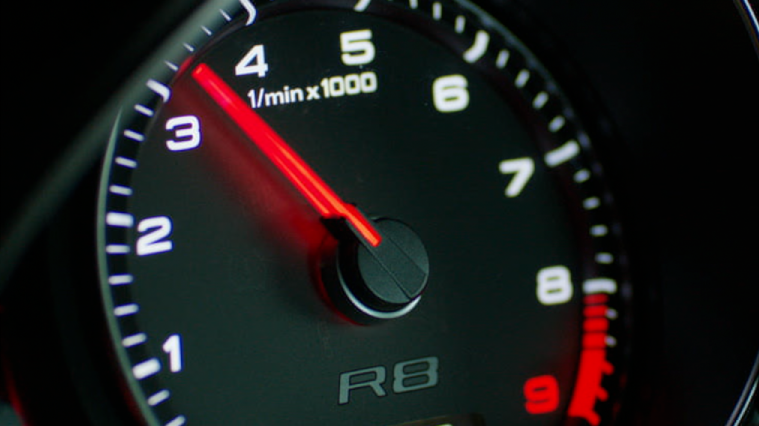
\includegraphics[height=2.8cm]{luma_fill}}
    \subfigure[Luma keyed image]{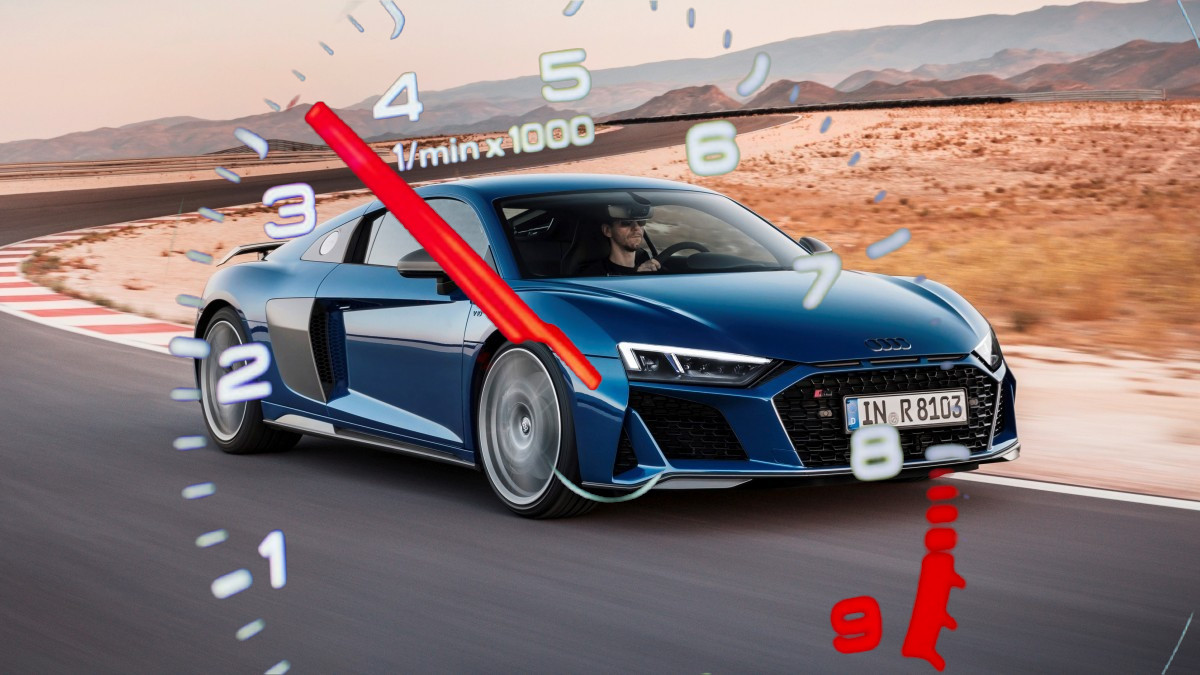
\includegraphics[height=2.8cm]{luma_comp}}

    \caption{Luma key example}
    \label{fig:02:luma_key_example}
\end{figure}

\subsubsection{Chroma keying}
As opposed to luma keying, chroma keying uses the color information of a video signal to discriminate the transparent and opaque parts of an image. In this case, the obtaining of the control signal is more complex and highly implementation dependant, so it will not be described here. However, it is worth mentioning that it should be done in a color model where the color information is explicit, as is the case of YUV, YIQ, YCbCr, YCtCp, HSV or HSL.\newline

This keying is sometimes referred as the \textit{green-screen effect}, as it is usually configured to reject the green color\cite{OrtizRodriguez2018}. Historically, its most widespread usage has been in weather forecasts, where the presenter gets overlaid in front of a weather map. The green color is commonly used because it rarely appears on skin-tones and costumes. However, if this is the case, a blue screen is used instead. The example shown in the figure \ref{fig:02:chroma_key_example} makes a more creative use of this effect, as it uses green suits on purpose.\newline

\begin{figure}[htbp]
    \centering
    \subfigure[Background image]{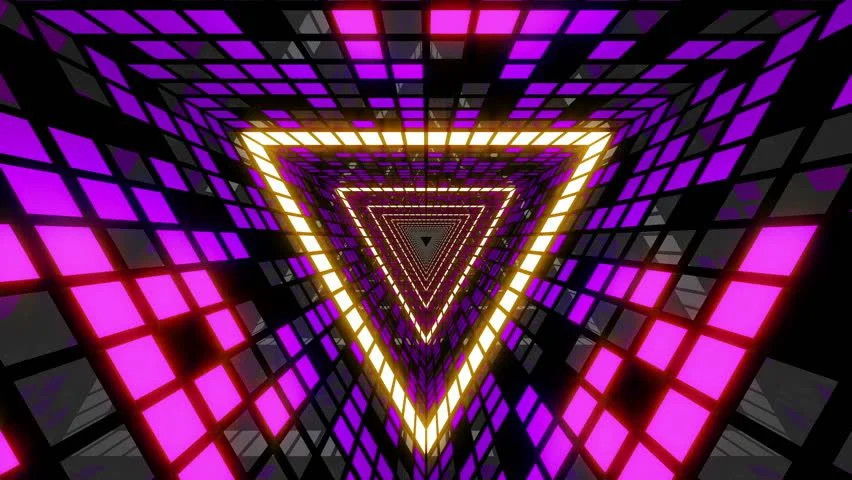
\includegraphics[height=2.8cm]{chroma_bkgd}}
    \subfigure[Key source]{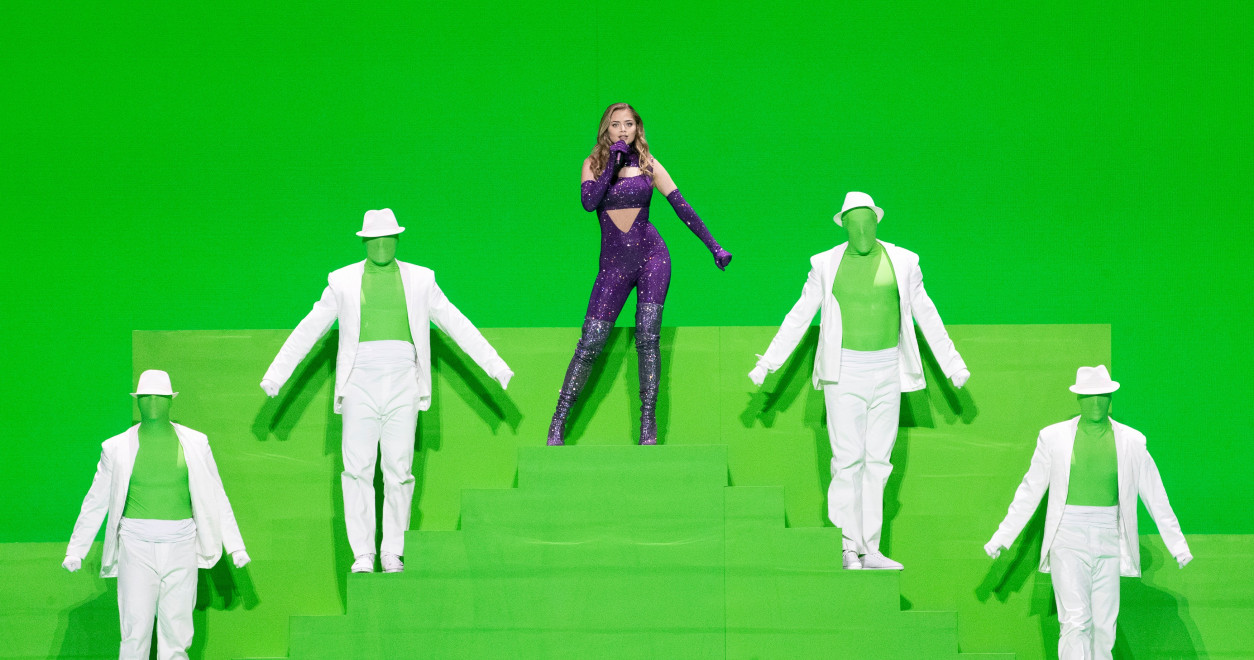
\includegraphics[height=2.8cm]{chroma_fill}}
    \subfigure[Chroma keyed image]{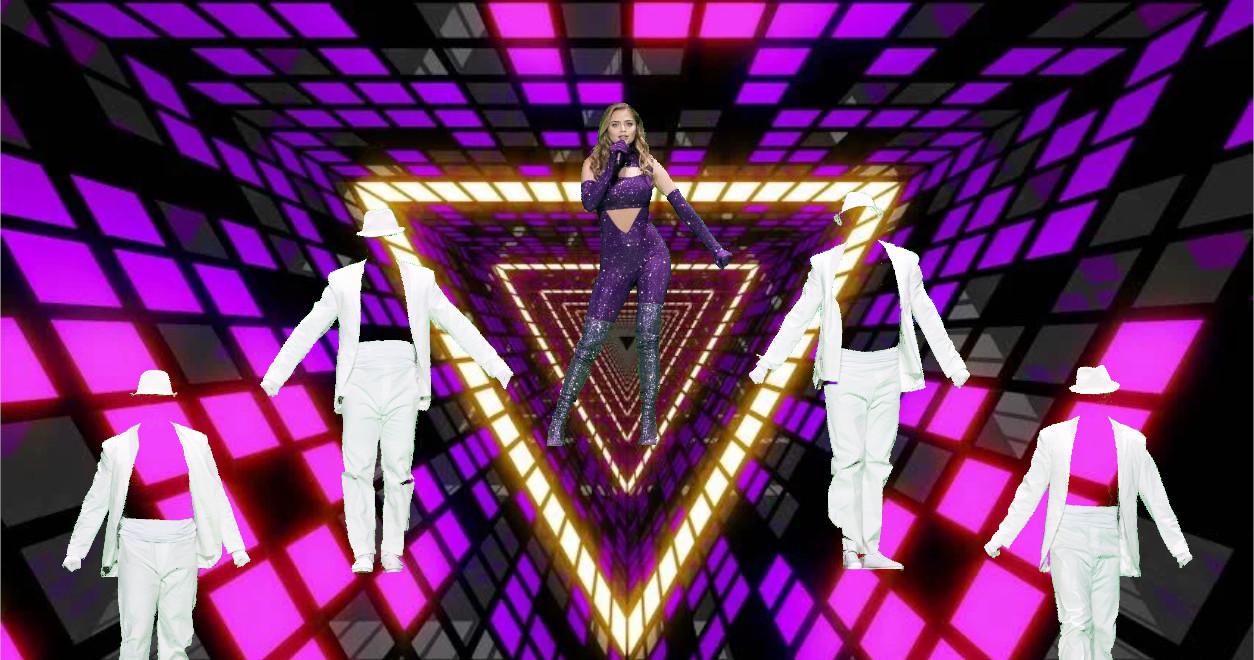
\includegraphics[height=2.8cm]{chroma_comp}}

    \caption{Chroma key example}
    \label{fig:02:chroma_key_example}
\end{figure}

\subsubsection{DVEs}
DVE stands for Digital Video Effects. Although modern mixers are fully digital, this name dates to the analog mixers, when certain effects could not be achieved with analog circuitry. Mainly, this refers to the ability to perform geometrical transformations on an overlay, such as scaling, rotating and positioning it in space. For example both \glspl{usk} in the figure \ref{fig:02:usk_dsk_example} are using a \gls{dve}. Among all the keying techniques described here, this is the only one that can not be modelled using the mixing equation, although some implementations may use it to embed the transformed image into the background\cite{OrtizRodriguez2018}.\newline

It is usually paired with animation controls, as it is useful to give dynamism to these effects. Moreover, it may offer the ability to generate borders around the transformed frame\cite{atemManual} and perform complex spatial transformations like 3D effects\cite{xvsManual}.\newline

\subsection{Transitions}
As mentioned earlier, \glspl{me} have two compositing buses which can be swapped with a transition. This transition is applied to the signal that carries the background information with the \glspl{usk} overlaid. Mixers offer a wide range of transition effects, the most basic of which will be explained hereafter.\newline

Similarly to keyers, most transition effects also use the mixing equation \eqref{eq:mixing}. However, as opposed to keyers where the control signal is generated from an external source (except for the pattern keying), transition's control signal is internally generated and depends on the progress of the transition. This progress will be denoted with $t \in [0, 1]$. Therefore, the control signal will also be a function of the progress: $c(x, y, t)$.\newline

From the operator's point of view, the progress of the transition can be controlled in two manners. The first one is pressing the automatic transition button. This will animate the $t$ parameter to travel from $0$ to $1$ in a preconfigured amount of time. The other way is to manually animate the $t$ parameter using a potentiometer. This potentiomenter is usually referred as the \textit{T-bar} due to its characteristic 'T' shape, as shown in the figure \ref{fig:02:tbar}.\newline

\begin{figure}[htbp]
    \centering
    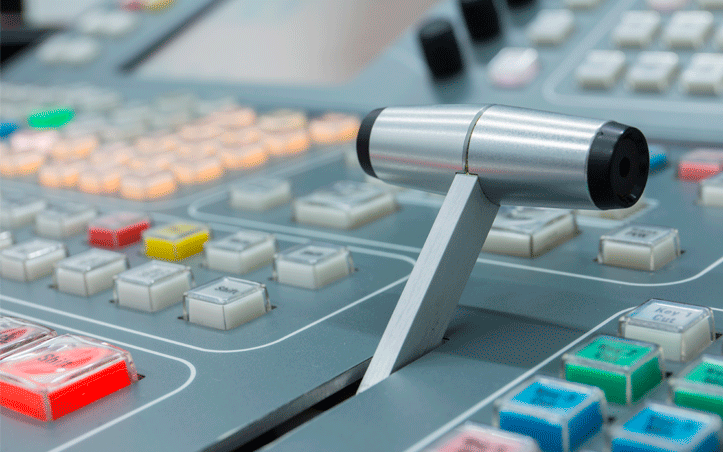
\includegraphics[width=.8\textwidth]{T Bar}
    \caption{\textit{T-bar} of a Grass Valley Kayak 1 M/E vision mixer}
    \label{fig:02:tbar}
\end{figure}

\subsubsection{Mix}
This is the most basic transition effect. It consists in steadily fading from one source to another, as displayed in the figure \ref{fig:02:mix_transition_example}. In its most basic form, it can be modelled using a control signal that is constant throughout the frame: $c(x, y, t) = t$.\newline

\begin{figure}[htbp]
    \centering
    \includegraphics[width=\textwidth]{Mix Transition AB}
    \caption{Mix transition example}
    \label{fig:02:mix_transition_example}
\end{figure}

Some mixers have the ability to transition from one feed to another passing through a third source, as illustrated by the figure \ref{fig:02:dip_transition_example}. This can be considered two mix transitions executed one after the other. Although the middle image can be anything, more often than not, it is a solid color\cite{atemManual}.\newline

\begin{figure}[htbp]
    \centering
    \includegraphics[width=\textwidth]{Dip Transition AB}
    \caption{Dip transition example}
    \label{fig:02:dip_transition_example}
\end{figure}

\subsubsection{Wipe}
As opposed to the previous transition, this one uses a control signal that is not the same for all \glspl{pixel} of an image. As the shape of this signal can be arbitrary, this leads to a wide fan of possible variants for this kind of transitions. Some example patterns are shown in the figures \ref{fig:02:wipes} and \ref{fig:02:wipe_transition_example}. The generation of these patterns is usually similar to the patterns described for pattern keying.\newline

\begin{figure}[htbp]
    \centering
    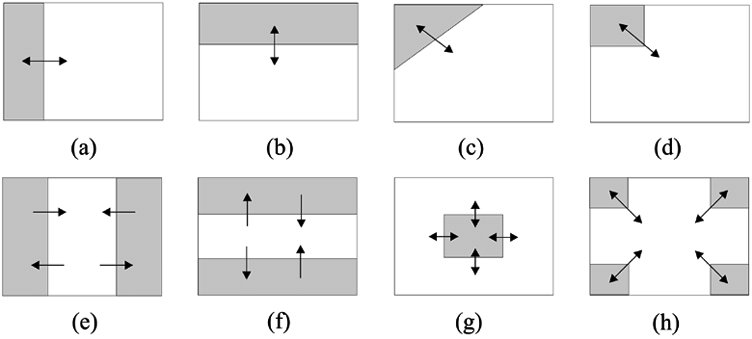
\includegraphics[width=.6\textwidth]{Wipes}
    \caption{Typical wipe transition patters}
    \label{fig:02:wipes}
\end{figure}

\begin{figure}[htbp]
    \centering
    \includegraphics[width=\textwidth]{Wipe Transition AB}
    \caption{Wipe transition example}
    \label{fig:02:wipe_transition_example}
\end{figure}

\subsubsection{DVE-based}
\Gls{dve} transitions treat the in-going and out-going feeds as overlays where at least one of them has an animation which makes is appear or disappear from the screen. Obviously, the the usage of \gls{dve} effects implies that it will not use the mixing equation. Similarly to wipe patterns, \gls{dve} transitions also have many possible animations. An example of one of them is displayed in the figure \ref{fig:02:dve_transition_example}.\newline

\begin{figure}[htbp]
    \centering
    \includegraphics[width=\textwidth]{DVE Transition AB}
    \caption{DVE transition example}
    \label{fig:02:dve_transition_example}
\end{figure}

\section{Software based vision mixers}
Recent increases in computational power have led to the possibility of manipulation video using software tools. This brings up the possibility of emulating the vision mixers described earlier using computer software. In essence, this allows using any computer for live video production, something that previously could only be done using dedicated equipment\cite{wikiSoftware_vision_mixer}.\newline

With the purpose of achieving the maximum performance, software-based vision mixers use \gls{gpu} acceleration, this is, they use computer's dedicated graphics processing hardware to offload image processing from the \gls{cpu}. The main limiting factor will be bit-rates across different buses of the computer, which will impact the maximum amount of sources that can be handled by a given machine.\newline

All vision mixers need to be able to ingest/output video from/to external sources, such as cameras. Most mixers do this though the \gls{sdi} interface. In order to do this using a software solution, the host computer must feature a \gls{sdi} \gls{io} card. However, if this is not present, network based solutions exist, namely, \gls{ip} based production. Moreover, all computers can output video though the graphic card's consumer-grade video outputs. Therefore, in a \gls{ip} based production environment, any computer can play the role of the vision mixer.\newline



\subsection{Existing solutions}
According to experts, the first software mixer was NewTek's Amiga Video Toaster, released in 1990. However, this was an expansion card for the Amiga 2000 computer which implemented a hardware vision mixer alongside a companion app, defeating many purposes of software vision mixers. Nevertheless, it allowed to produce video in a centralized manner, converging in the same machine a 4 channel vision mixer and a \gls{cg}. It was not until 2005 when this same company introduced its TriCaster line of products\cite{neoteoAmigaVideoToaster}. NewTek TriCasters are a hardware solution, but under the hood they are built with off-the-shelf \gls{pc} parts and video \gls{io} cards.\newline

Many traditional brands have moved towards NewTek's first approach, this is, the integration of mixer-specific hardware inside \glspl{pc}. The primary advantage of this is that the most part of handling video can be done in hardware, allowing to obtain a higher throughput whilst keeping the flexibility of software-based solutions. A example of this approach is Ross' Graphite line of products, that as seen in the figure \ref{fig:02:ross_graphite} is based on a standard \gls{pc} motherboard with a proprietary PCIe expansion card\cite{graphiteManual}.\newline

\begin{figure}[htbp]
    \centering
    \subfigure[I/O of the mixer]{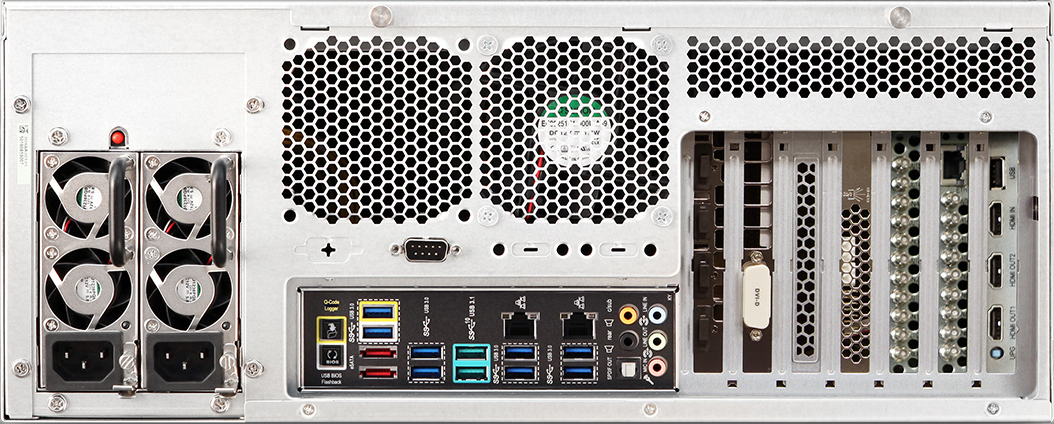
\includegraphics[height=5cm]{graphite_frame_back}}
    \subfigure[Add-on PCIe card]{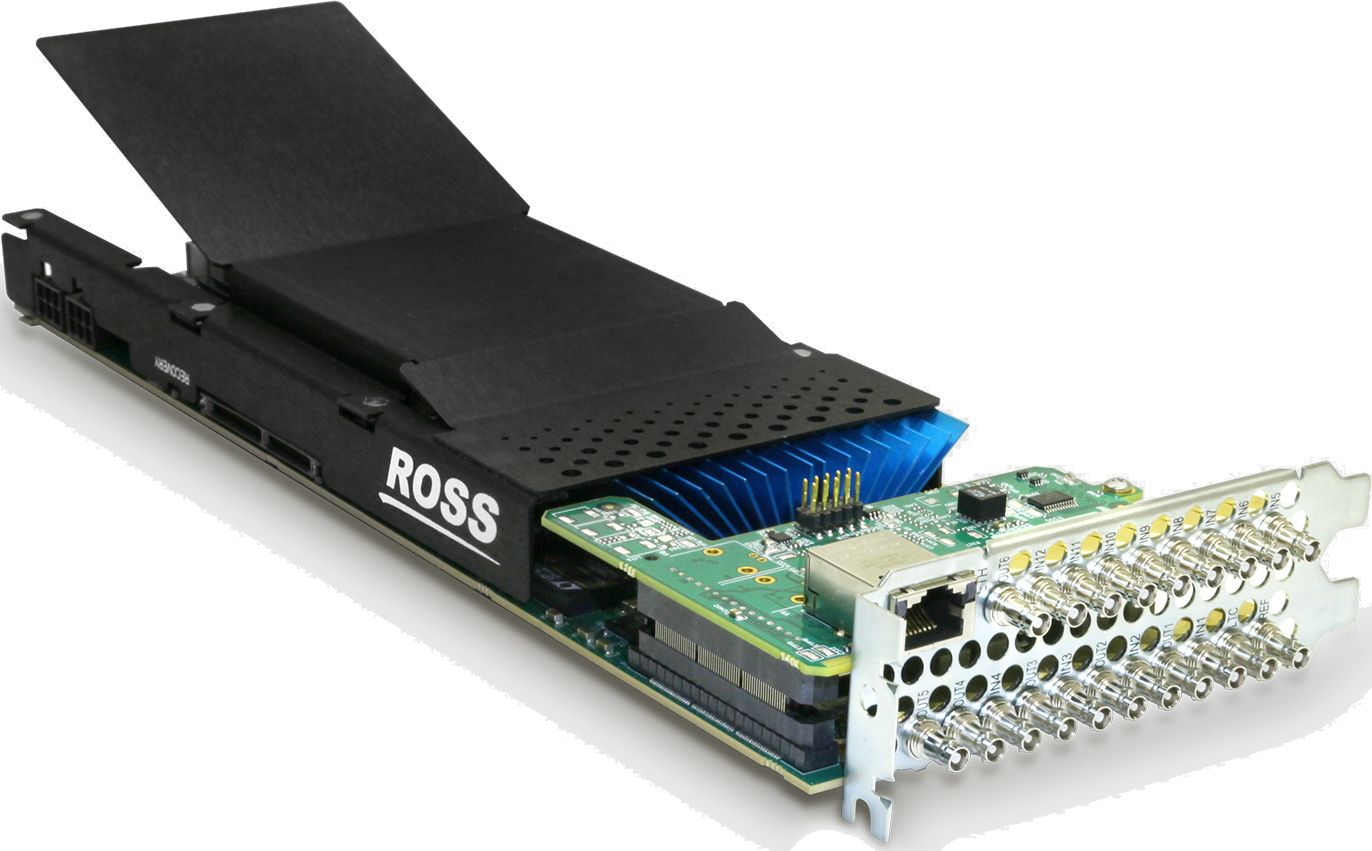
\includegraphics[height=5cm]{graphite_pcie_card}}

    \caption{Ross Graphite vision mixer}
    \label{fig:02:ross_graphite}
\end{figure}

Later in 2010, another company called vMix emerged with a video switching software which could be run on any hardware. As of writing this report, this software still exists and its developers have been pushing new releases periodically.\newline

The next year, in 2011, the first version of \gls{obs} was released, which at the time was a simple \gls{foss} video streaming tool. After years of development, this software has evolved into a scene-based vision mixer with lots of features and \gls{io} capabilities\cite{obsWiki}. Its main users are streamers, which more often than not have modest video production requirements such as embedding their webcam in the screen for streaming it to popular streaming platforms.\newline

Another related solution is CasparCG, a general purpose \gls{foss} \gls{cg}, developed by the \gls{svt}. Although it is not strictly a vision mixer, it has been included here because it can not only output video, but also consume it and perform complex compositions with it, as seen in the figure \ref{fig:02:casparcg}. According to its authors, it could be used as a vision mixer, but this is not its intended operating purpose. It powers many broadcasts produced by members of the \gls{ebu}\cite{casparcgWiki}.\newline

\begin{figure}[htbp]
    \centering
    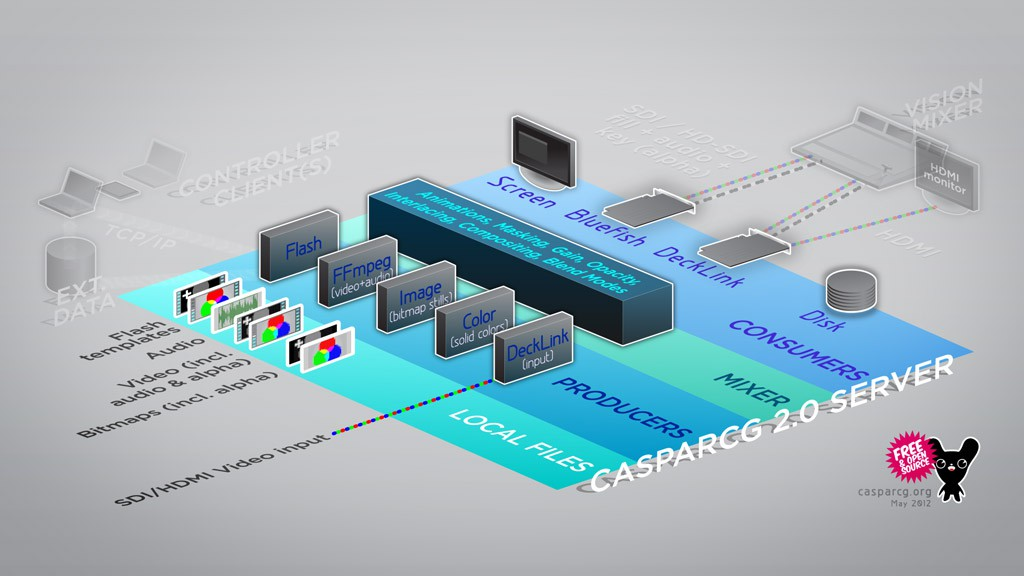
\includegraphics[width=\textwidth]{CasparCG}
    \caption{CasparCG's architecture}
    \label{fig:02:casparcg}
\end{figure}

\subsection{Benefits and drawbacks}
The major benefits of using software solutions are the cost savings and their flexibility. Even considering the cost of a high-end workstation with multiple \gls{sdi} \gls{io} cards, it will easily outperform a higher prized hardware solution in terms of composition capabilities. Moreover, software-based vision mixers tend to integrate many other production systems such as \glspl{cg}, media players, virtual set generators, etc\dots\cite{tricasterManual}\cite{vmixManual}. This not only reduces the cost on auxiliary equipment, but also its own physical \gls{io} requirements.\newline

What is more, computational resources can be dynamically allocated. For instance, the same computer may be used to produce a simple \gls{uhd} show or to perform a very complex \gls{fhd} compostion, or even multiple \gls{fhd} compositions. As opposed to this, hardware mixers have dedicated resources for dedicated tasks. This means that for the previous example, a buyer would need to choose a \gls{uhd} mixer capable of producing multiple complex compositions, even if it is not going to use all features simultaneously.\newline

However, software-based vision mixers also present some drawbacks. First of all, the latency is orders of magnitude higher. For istance, Black Magick Atem switchers have a latency lower than one scan-line when genlocked\cite{atemManual} ($\approx 30 \si{\micro\second}$ for 1080p30), whilst software solutions have latencies in the neighborhood of a few frames\cite{tricasterManual} ($\approx 66 \si{\milli\second}$ for the same situation). This last number rubs the the delays noticeable by human brains. Therefore, this makes them inadvisable for use cases where the audience has other means of sensory input, as is the case of image magnification in a concert, as shown in the figure \ref{fig:02:imag}. For the rest of broadcast use cases, this is not a serious concern.\newline

\begin{figure}[htbp]
    \centering
    \includegraphics[width=.8\textwidth]{Weezer image magnification}
    \caption{Image magnification in a Weezer's concert}
    \label{fig:02:imag}
\end{figure}

Another drawback is that software-based solutions are not as reliable as hardware-based ones. As broadcasting equipment is produced with very high quality standards, physical vision mixers are virtually unbeatable, being able to run 24/7 for years with very low maintenance, as long as they are protected against power outages with a \gls{ups}. As opposed to this, software-based mixers are susceptible to software-bugs, \gls{os} updates, etc\dots This last concern rules out using them for continuity control.\newline

Finally, current computers can not meet the input requirements of large-scale shows. However, as computer's internal bandwidths and computational power rise, this gap will become narrower, eventually disappearing.\newline

\section{IP based production}
As mentioned earlier, \gls{ip} based production consists in using standard computer networking infrastructures to transport video inside a \gls{tv} production facility. This is a very current topic, as many \gls{tv} stations are undergoing through a conversion from \gls{sdi} based infrastructures to \gls{ip} based ones\cite{tmRtveIp}.\newline

As opposed to the traditional streaming, \gls{ip} based production must meet some additional requirements. For instance, the quality of the image must be comparable to the quality provided by uncompressed \gls{sdi}. This rules out using any heavy compression algorithms. Moreover, the latency must be as low as possible, making it impossible to use bidirectional frame compression. Additionally, the signal must fit into a $1 \si{\giga b \per\second}$ or $10 \si{\giga b \per\second}$ link. Finally, it must be able to carry some ancillary data from and to the source.\newline

The first protocol to perform such a task was introduced in 2007 as the SMPTE-2022. This protocol allows sending a MPEG-2 stream or a packetized SD-\gls{sdi} ($270 \si{\mega b \per\second}$) stream over a $1 \si{\giga b \per \second}$ Ethernet cable\cite{tmIpProduction}. Later in 2017, this standard was upgraded to the SMPTE-2110, which brings many benefits, such as better synchronization mechanisms and support for any resolution, including those larger than \gls{uhd}, as long as there is enough bandwidth \cite{smpte2110faq}. The largest problem with the SMPTE-2110 protocol is that it is not meant to be used by computers, specially in the case of \gls{uhd} signals, as the bitrate is too high for modern \glspl{cpu}.\newline

Another proliferating protocol is NewTek's \gls{ndi}, which is a royalty-free standard. As opposed to SMPTE's \gls{ip} based production protocols, it is paired with a intra-frame compression codec, although it is able to transport existing video codecs such as H.264 and H.265. This makes it possible to use it with standard networking gear and modest computers whilst keeping resolutions up to \gls{uhd}. Their own codec has been designed to meet the quality requirements mentioned earlier.\newline

%Print bibliography if it is being compiled standalone
%\printbibliography

\end{document}
